% This work is licensed under the Creative Commons Attribution-NonCommercial 4.0 International License.
% To view a copy of this license, visit http://creativecommons.org/licenses/by-nc/4.0/
% or send a letter to Creative Commons, PO Box 1866, Mountain View, CA 94042, USA.

% !TEX TS-program = xelatex	

\documentclass[../Main/chem532-notes.tex]{subfiles}

\begin{document}

\setcounter{chapter}{9}

\chapter{Multireference wave function methods}
In this chapter we will discuss methods can be used to treat bond break process and electronically excited states.

\section{Multiconfigurational self-consistent-field theory}

As we have seen previously, in many cases the Hartree--Fock method is usually captures a large fraction of the total electronic energy.
This is usually true of closed-shell molecules and high-spin open-shells.
However, we have also encountered cases, like for example, the \ce{H2} molecule the dissociation limit, where a single determinant wave function fails to capture even the correct qualitative behavior of the electrons.

In this section we will discuss multiconfigurational self-consistent-field (MCSCF) methods, which may be viewed as generalizations of Hartree--Fock theory.
In MCSCF methods, an electronic state is approximated with a small configuration interaction wave function
\begin{equation}
\ket{\Psi_\mathrm{MCSCF}} 
= \sum_I C_I \ket{\Phi_I},
\end{equation}
 in which both the orbitals ($\phi_i$) from which the determinants ($\Phi_I$) and the determinant coefficients ($C_I$) are variationally optimized.
Note, that in general, that they determinants employed to expand the MCSCF wave function (understood as occupation patters of electrons) are not changed in the optimization process.
 
The MCSCF energy is obtained by performing a simultaneous optimization of the orbitals and the determinant coefficients
\begin{equation}
E_\mathrm{MCSCF} = \min_{C_I, \{ \psi_i \}}\braket{\Psi_\mathrm{MCSCF} | \hat{H} | \Psi_\mathrm{MCSCF}},
\end{equation}
imposing that the determinant vector is normalized ($\sum_I |C_I|^2 = 1$) and the orbitals are orthonormal.
It is always implicitly assumed that the MCSCF wave function is constructed using restricted spin orbitals so that the alpha and beta spatial parts of a given orbital are the same.

Different MCSCF methods are defined by the way the determinant are selected.
The most widely used approach is the complete-active-space self-consistent-field (CASSCF) method, which basically forms all the MCSCF determinant by performing a FCI in a limited number of orbitals.
In CASSCF one starts by partitioning the orbitals into three spaces:
\begin{itemize}
\item \textbf{Core (or doubly occupied) orbitals ($\mathbf{C}$)}. These orbitals are generally the lowest one in energy and are kept doubly occupied in all the determinants in the CASSCF wave function.
\item \textbf{Active orbitals ($\mathbf{A}$)}. These orbitals have variable occupation in the CASSCF wave function. In most cases these are chosen to be valence orbital associated with the particular aspect we want to model. For example, for to describe the wave function for the single bond-breaking reaction \ce{A-B -> A + B} it is sufficient to include a single pair of \ce{A-B} bonding/antibonding orbitals.
\item \textbf{Virtual orbitals ($\mathbf{V}$)}. These orbitals are not occupied in the CASSCF wave function. These are usually high-energy orbitals that are typically irrelevant to description of a chemical reaction or an excited state. 
\end{itemize}

\begin{center}
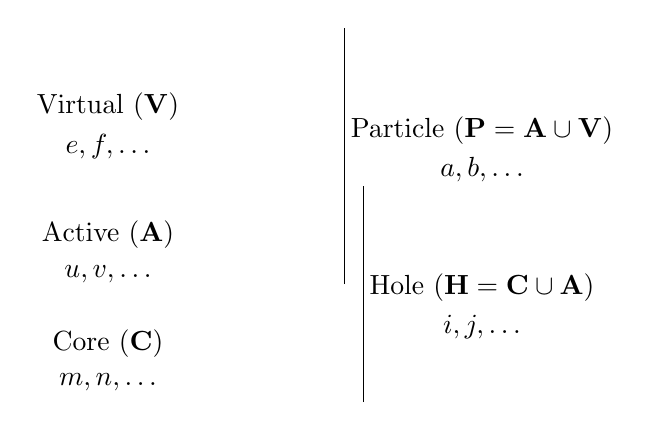
\begin{tikzpicture}[] 
\draw (0,0.5) node{Core ($\mathbf{C}$)};
\draw (0,0.) node{$m, n, \ldots$};
\draw (0,1.875) node{Active ($\mathbf{A}$)};
\draw (0,1.375) node{$u, v, \ldots$};
\draw (0,3.5) node{Virtual ($\mathbf{V}$)};
\draw (0,3.0) node{$e, f , \ldots$};
\draw (4.75,1.2) node{Hole ($\mathbf{H} = \mathbf{C} \cup \mathbf{A}$)};
\draw (4.75,0.7) node{$i,j,\ldots$};
\draw (3.25,-0.25) -- (3.25,2.5);
\draw (4.75,3.2) node{Particle ($\mathbf{P} = \mathbf{A} \cup \mathbf{V}$)};
\draw (4.75,2.7)  node{$a,b,\ldots$};
\draw (3,1.25) -- (3,4.5);
\mo{0.0} \mo{0.25} \mo{0.5} \mo{0.75} \mo{1.0}
\mo[gray]{1.5} \mo[gray]{1.75} \mo[gray]{2.0} \mo[gray]{2.25}
\mo[none]{2.75} \mo[none]{3.00} \mo[none]{3.25} \mo[none]{3.50}
\mo[none]{3.75} \mo[none]{4.0} \mo[none]{4.25}
\end{tikzpicture}
\end{center}

In CASSCF one generates determinants with the core orbitals occupied and $n_\mathbf{A}$ active electrons distributed in the active orbitals.
Therefore, a generic CASSCF determinant has the form
\begin{equation}
\ket{\Phi_I} = \underbrace{\cop{u} \cop{v} \cdots  \cop{z}}_{\text{active}} \prod_m^\mathbf{C} \cop{m} \ket{}.
\end{equation}
In the literature, and active space in which a given number of electrons ($n_\mathrm{el}$) is distributed in a given number of active orbitals ($n_\mathbf{A}$) is abbreviated with CAS($n_\mathrm{el}$e,$n_\mathbf{A}$o).
For example, an active space with two electrons in two orbitals is denoted CAS(2e,2o).

In CASSCF, the space of determinants is \textbf{complete}, in the sense that all possible determinants are included.
One consequence of this choice is that the wave function is invariant with respect to unitary transformations of the active orbitals.
This means that if we transform the active orbitals via a unitary transformation $\mathbf{U}$
\begin{equation}
\psi_u \rightarrow \psi'_u = \sum_v \psi_v U_{vu},
\end{equation}
and consequently all the determinant change according to
\begin{equation}
\ket{\Phi_I} = \ket{\psi_{i_1} \psi_{i_2} \cdots \psi_{i_N}}
\rightarrow  \ket{\Phi'_I} = \ket{\psi'_{i_1} \psi'_{i_2} \cdots \psi'_{i_N}},
\end{equation}
there is a corresponding set of CI coefficients $C'_I$ such that the transformed CASSCF wave function is identical to the original one
\begin{equation}
\sum_I C_I \ket{\Phi_I} = \sum_I C'_I \ket{\Phi'_I}.
\end{equation}
This property implies that we are free to work with any unitarily transformed version of the CASSCF active orbitals (e.g., delocalized, localized).

Note that since the CAS space includes all possible determinants, its size grows very quickly with the number of active orbitals and electrons.
If we ignore point group symmetry, we can compute the number of determinants with a given number of alpha ($n_\alpha$) and beta ($n_\beta$) electrons in the active orbitals just by counting how many arrangements of electrons are possible for the two spin cases.
For each spin case, the number of ways we can distribute $n$ electrons is given by the number of ways we can choose $n$ spin orbitals to occupy and taking into account that permutations are equivalent.
This quantity is given by the binomial coefficient
\begin{equation}
\binom{n}{k} = \frac{n!}{(n-k)! k!},
\end{equation}
where $n! = 1 \times 2 \times \ldots \times n$, and $0! = 1$ by definition.
The total number of determinants ($d$) is given by the product of the number of arrangements of alpha and beta electrons
\begin{equation}
d = \binom{n_\mathbf{A}}{n_\alpha} \binom{n_\mathbf{A}}{n_\beta}.
\end{equation}
As shown in Tab.~\ref{tab:cas_size}, this quantity grows very quickly, and therefore, practical computations are typically limited to active spaces of size CAS(16e,16o).

% Requires the booktabs if the memoir class is not being used
\begin{table}[htbp]
   \centering
   %\topcaption{Table captions are better up top} % requires the topcapt package
   \begin{tabular}{@{} lcr @{}} % Column formatting, @{} suppresses leading/trailing space
      \toprule
      \multicolumn{2}{c}{Size of the active space} \\
      \cmidrule(r){1-2} % Partial rule. (r) trims the line a little bit on the right; (l) & (lr) also possible
      Active electrons    & Active orbitals & CAS determinants\\
      \midrule
      2 & 2 & 4 \\
      4 & 4 & 36 \\
      6 & 6 & 400 \\
      8 & 8 & 4,900 \\
      10 & 10 & 63,504 \\
      12 & 12 & 853,776 \\
      14 & 14 & 11,778,624 \\
      16 & 16 & 165,636,900 \\
      18 & 18 & 2,363,904,400 \\
      20 & 20 & 34,134,779,536 \\
      \bottomrule
   \end{tabular}
   \caption{Number of determinants in a CAS space at half filling. These numbers ignore the reduction in size due to point group symmetry.}
   \label{tab:cas_size}
\end{table}

Note that one can also define a corresponding CASCI approach in which one generated a CAS space and performs the variational optimization of the CI coefficients \textbf{without} optimizing the orbitals.

\section{Multireference configuration interaction}
The CASSCF method can only account for static correlation effects, which in practice is not enough to accurately describe multideterminantal electronic states.
The simplest way to include dynamical correlation effects on top of a CASSCF reference is via a configuration interaction wave function.
In the multireference configuration interaction (MRCI) approach, one starts with a CASSCF reference and adds excited determinants that account for dynamical correlation effects.
The simplest approach is \textbf{uncontracted} MRCI with singles and doubles (u-MRCISD), in which one simply augments the CASSCF determinant space with all singly and doubly excited determinants of each reference determinant.
The u-MRCISD wave function is given by
\begin{equation}
\ket{\Psi_\text{u-MRCI}}  
= \sum_I^{\mathrm{CAS}} C_I \ket{\Phi_I} + \sum_A^{\mathrm{EXT}} C_A \ket{\Phi_A},
\end{equation}
where the space of external determinants is generated by applying the operators $\cop{a} \aop{i}$ and $\cop{a} \cop{b} \aop{j} \aop{i}$ to all the CAS determinants
\begin{equation}
\mathrm{EXT} = \{ \Phi_A | \Phi_A = \cop{a} \aop{i} \ket{\Phi_I}, 
\cop{a} \cop{b} \aop{j} \aop{i} \ket{\Phi_I} \forall \Phi_I \in \mathrm{CAS}\}.
\end{equation}
In defining the EXT space, the orbital indices $i,j$ run over the core and active orbitals, while $a,b$ run over the active and virtuals.
The u-MRCISD method provides very accurate results, but it has a computational scaling that becomes quickly unmanageable when the number of CAS determinants is large.
The approximate number of u-MRCISD determinants depends on the number of hole ($N_\mathrm{H}$) and particle ($N_\mathrm{P}$) orbitals and is proportional to
\begin{equation}
N_\mathrm{det}^\text{u-MRCISD} = d N_\mathrm{H}^2 N_\mathrm{P}^2,
\end{equation}
which is limited both by the size of the active space ($d$) and the number of electrons and basis functions used.

A more economical alternative to the u-MRCISD method is the \textbf{internally-contracted} MRCISD (ic-MRCISD) method.
In ic-MRCISD, one still generates all possible singles and doubles out of a CAS; however, an excitation operator is applied to the entire CAS reference all at once.
For example, internally-contracted singly excited configurations are defined as
\begin{equation}
\ket{\Psi_{i}^{a}} = \cop{a} \aop{i} \ket{\Psi_\mathrm{CAS}} =  \sum_I C_I \cop{a} \aop{i}\ket{\Phi_I}.
\end{equation}
The right hand side of this equation shows that $\ket{\Psi_{i}^{a}}$ is a linear combination of excited determinants ($\cop{a} \aop{i}\ket{\Phi_I}$) with coefficients fixed to the value of the CAS wave function ($C_I$).

The ic-MRCISD wave function is defined by the following wave function guess
\begin{equation}
\begin{split}
\ket{\Psi_\text{ic-MRCISD}}  
= & (1 + \hat{C}) \ket{\Psi_\mathrm{CAS}} \\
= & \sum_I C_I \ket{\Phi_I} + \sum_{i}\sum_{a} c_{i}^{a} \cop{a}\aop{i} \ket{\Psi_\mathrm{CAS}}
+ \frac{1}{4} \sum_{ij}\sum_{ab} c_{ij}^{ab}  \cop{a}\cop{b}\aop{j}\aop{i} \ket{\Psi_\mathrm{CAS}} \\
= & \sum_I C_I \ket{\Phi_I} + \sum_{i}\sum_{a} c_{i}^{a} \ket{\Psi_{i}^{a}}
+ \frac{1}{4} \sum_{ij}\sum_{ab} c_{ij}^{ab} \ket{\Psi_{ij}^{ab}},
\end{split}
\end{equation}
where the coefficients $c_{i}^{a}$ and $c_{ij}^{ab}$ are obtained by minimizing the energy of the ic-MRCISD wave function.
Therefore, the number of variational parameters in the ic-MRCISD wave function is of the order of $N_\mathrm{H}^2 N_\mathrm{P}^2$, which is significantly less than the corresponding  for u-MRCISD.
The lower scaling of  ic-MRCISD makes it the methods of choice among all variants of MRCI.
Note, however, that there are several very important variants of MRCI that only partially contract the wave function.

\section{Multireference perturbation theory and coupled cluster theory}

It is also possible to generalize perturbation theory to the case of a multideterminantal reference.
As for standard M{\o}ller--Plesset perturbation theory, one has to select a partitioning of the Hamiltonian into zeroth- plus first-order terms.
In the case of multideterminantal references this choice is not straightforward and several choices have been considered.
The simplest strategy is to employ a \textbf{diagonal} one-body zeroth-order operator, like in M{\o}ller--Plesset perturbation theory, for example
\begin{equation}
\hat{H}_0 = \sum_{p} \epsilon_p \cop{p}\aop{p},
\end{equation}
however, a more common choice employs a general one-body operator
\begin{equation}
\hat{F} = \sum_{pq} f_{pq} \cop{p}\aop{p},
\end{equation}
where $ f_{pq}$ are matrix elements of the average Fock matrix and are computed as
\begin{equation}
 f_{pq} = \braket{\Psi^{(0)} | [\aop{p}, [\hat{H},\cop{q}]]_+|\Psi^{(0)}}.
 \end{equation}
 Then the corresponding zeroth-order Hamiltonian is expressed as
 \begin{equation}
\hat{H}_0 = \hat{P}_\mathrm{CAS} \hat{H} \hat{P}_\mathrm{CAS} 
+ \hat{P}_\mathrm{SD} \hat{F} \hat{P}_\mathrm{SD},
\end{equation}
where $\hat{P}_\mathrm{CAS}$ and $\hat{P}_\mathrm{SD}$ are projection operators defined in terms of the CAS determinants and all singly and doubly excited determinants generated from the CAS (SD). For example, $\hat{P}_\mathrm{CAS}$ is defined as
\begin{equation}
\hat{P}_\mathrm{CAS} = \sum_I^\mathrm{CAS} \ket{\Phi_I}\bra{\Phi_I}.
\end{equation}
Another way to define $\hat{F}$ is using the Dyall partitioning, which includes two-body terms in the active space.
Note that it was also found beneficial to apply a shift to the active orbital energies (IPEA shift) to 

Like for MRCI, one can develop various contracted variants of MRPT: uncontracted, partially-contracted, internally-contracted, and strongly contracted. All of these differ in the number of variational degrees of freedom.
The most common formulation of MRPT are the second-order CAS perturbation theory (CASPT2) and second-order $n$-electron valence perturbation theory (NEVPT2).
Describing these approaches in detail is beyond the scope of these notes and the interested reader is urged to consult the primary literature.

Many variants of multireference coupled cluster (MRCC) methods have also been proposed.
These can be divided in four broad categories. The first is Fock-space multireference coupled cluster methods, which aim to describe states with different number of electrons.
The second one is Jeziorksi--Monkhorst methods, which employ an uncontracted ansatz of the form
\begin{equation}
\ket{\Psi_\text{JM-MRCC}}  = \sum_I^\mathrm{CAS} C_I e^{\hat{T}^I}\ket{\Phi_I}.
\end{equation}
The third type is internally-contracted MRCC theories, which generalize the ic-MRCI method and are based on the following ansatz
\begin{equation}
\ket{\Psi_\text{ic-MRCC}}  = e^{\hat{T}} \ket{\Psi_\mathrm{CAS}} 
= \sum_I^\mathrm{CAS} C_I e^{\hat{T}}\ket{\Phi_I}.
\end{equation}
There are also a large number of methods that use the single-reference CC ansatz but modify it so that it can describe some type of wave functions with mild multideterminantal character.
Some example include methods-of-moment CC, equation-of-motion spin-flip CC, and the CCSDt/CCSDtq methods.



\end{document}
